\documentclass[12pt]{article}


\usepackage{graphicx}
\usepackage{fullpage}

\setlength{\parindent}{0pt}
\setlength{\parskip}{1ex plus 0.5ex minus 0.2ex}


\begin{document}
\begin{center}
\textbf{
{ \LARGE CSE 834 -- Project} \\
Derek Weitzel \& Yutaka Tsutano
}
\end{center}

\section{Overview}
In this project, we will create a 16 bit low pass filter.  This filter is similar to those used in audio processing.  This specific properties of the filter where picked to simplify the design.

For each clock period, the circuit will:
\begin{itemize}
\item Shift the registers.  This will pop the last register's value, and save the data\_in value to the first register.
\item Calculate the convolution of the values inside the 8 registers.
\end{itemize}

The coefficients are fixed, therefore they will be constant in the multipliers, simplifying the design.  The input will be 1 bit for the clock, and 16 bits of input data.  The output will be the 16 bit output.  The format of the input and output will be Q15.  The multipliers  and registers will be done in VHDL in order to simplify design.

\begin{table}[ht]
\centering
\begin{tabular}{l | l | c}
\hline
Input/Output & Description & Bits \\
\hline \hline
Input & Clock & 1 \\
Input & Data In & 16 \\
Output & Convolution & 16 \\
\end{tabular}
\end{table}

We will tackle power concerns by optimizing the tree of adders (see Figure \ref{fig:diagram}).  Since we have a constant number of adders, we can create a large adder that will be able to minimize redundant gates.  Further, because of the symmetric property of the filter, we can minimize the number of multipliers by adding symmetric registers, then multiplying by the coefficient.  

\section{Timeline}

11/2 - 11/8: Registers and Multipliers \\
11/8 - 11/23: Optimized Adder \\
11/23 - 12/2: Report - Finalizations \\

\section{Filter Properties}
These are the specific filter properties that where used to calculate the Coefficients seen in Table \ref{tab:coefficients}.

Sampling Frequency Fs = 8194 Hz \\
Cut-off Frequency = 2048 Hz \\
FIR (Lowpass Filter with Hamming Window) \\

\begin{table}[ht]
\centering
\begin{tabular}{ c | r }
\hline
Coeffiecient & Value \\
\hline \hline
$C_0$ & -1.55107884796477e-18 \\
$C_1$ & -0.022663985459552 \\
$C_2$ & 1.04697822237622e-17 \\
$C_3$ & 0.273977082565524 \\
$C_4$ & 0.497373805788057 \\
$C_5$ & 0.273977082565524 \\
$C_6$ & 1.04697822237622e-17 \\
$C_7$ & -0.0226639854595526 \\
$C_8$ & -1.55107884796477e-18 \\
\end{tabular}
\caption{Coefficient values}
\label{tab:coefficients}
\end{table}


\begin{figure}[ht]
\centering
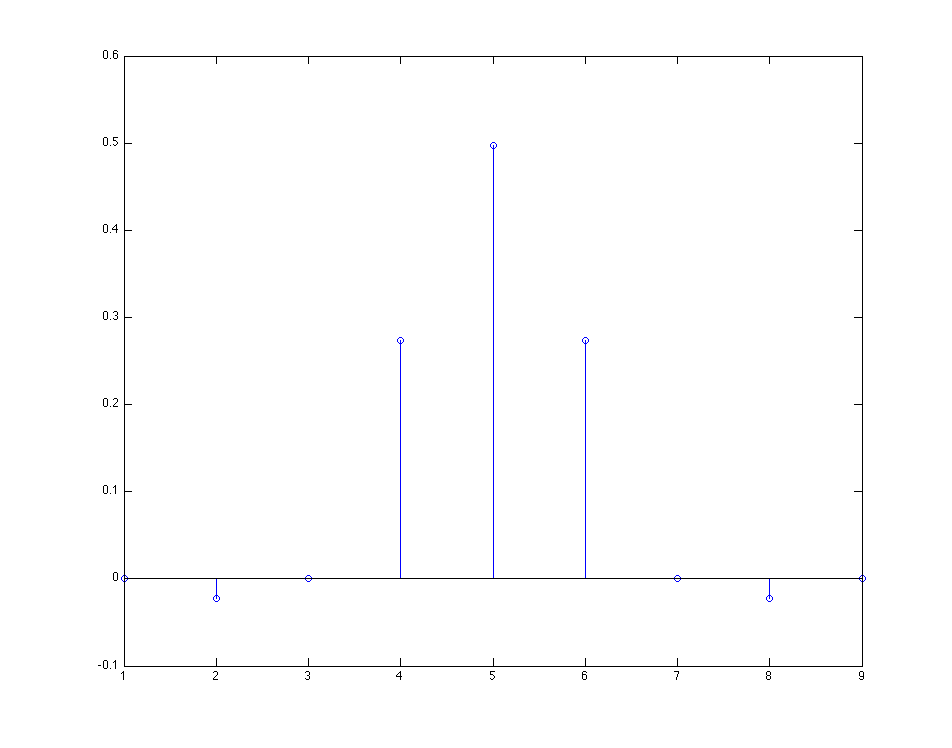
\includegraphics[scale=0.55]{../coeffs.png}
\caption{Plot of coefficients.  Notice the symmetry.}
\label{fig:plotcoefficients}
\end{figure}

\begin{figure}[ht]
\centering
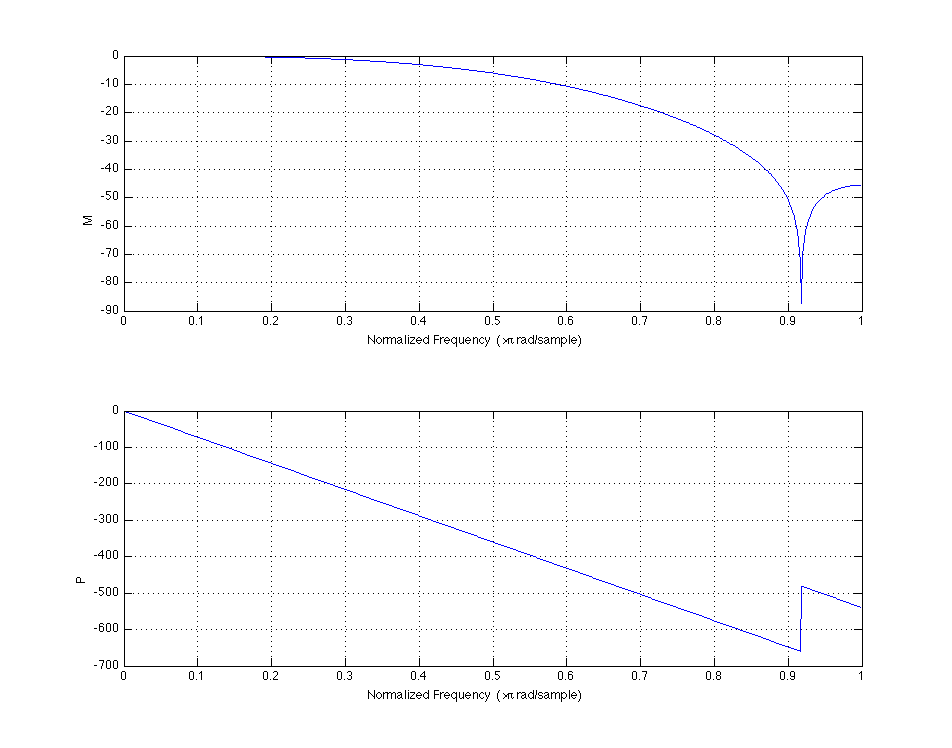
\includegraphics[scale=0.55]{../filter_design.png}
\caption{Plot of filter characteristics}
\label{fig:characteristics}
\end{figure}

\begin{figure}[ht]
\centering
\includegraphics[scale=0.55]{../Diagram.png}
\caption{Logical diagram of the data flow.}
\label{fig:diagram}
\end{figure}



\end{document}
